\documentclass[a4paper, 12pt]{article}

%%% Работа с русским языком
\usepackage{cmap}					% поиск в PDF
\usepackage{mathtext} 				% русские буквы в формулах
\usepackage[T2A]{fontenc}			% кодировка
\usepackage[utf8]{inputenc}			% кодировка исходного текста
\usepackage[russian]{babel}	% локализация и переносы

%%% Дополнительная работа с математикой
\usepackage{amsmath,amsfonts,amssymb,amsthm,mathtools} % AMS
\usepackage{icomma} % "Умная" запятая: $0,2$ --- число, $0, 2$ --- перечисление

%% Номера формул
%\mathtoolsset{showonlyrefs=true} % Показывать номера только у тех формул, на которые есть \eqref{} в тексте.

%% Шрифты
\usepackage{euscript}	 % Шрифт Евклид
\usepackage{mathrsfs} % Красивый матшрифт

%% Поля
\usepackage[left=2cm,right=2cm,top=2cm,bottom=2cm,bindingoffset=0cm]{geometry}

%% Русские списки
\usepackage{enumitem}
\makeatletter
\AddEnumerateCounter{\asbuk}{\russian@alph}{щ}
\makeatother

%%% Работа с картинками
\usepackage{graphicx}  % Для вставки рисунков
\graphicspath{{images/}{images2/}}  % папки с картинками
\setlength\fboxsep{3pt} % Отступ рамки \fbox{} от рисунка
\setlength\fboxrule{1pt} % Толщина линий рамки \fbox{}
\usepackage{wrapfig} % Обтекание рисунков и таблиц текстом

%%% Работа с таблицами
\usepackage{array,tabularx,tabulary,booktabs} % Дополнительная работа с таблицами
\usepackage{longtable}  % Длинные таблицы
\usepackage{multirow} % Слияние строк в таблице

%% Красная строка
\setlength{\parindent}{2em}

%% Интервалы
\linespread{1}
\usepackage{multirow}

%% TikZ
\usepackage{tikz}
\usetikzlibrary{graphs,graphs.standard}

%% Верхний колонтитул
\usepackage{fancyhdr}
\pagestyle{fancy}

%% Перенос знаков в формулах (по Львовскому)
\newcommand*{\hm}[1]{#1\nobreak\discretionary{}
	{\hbox{$\mathsurround=0pt #1$}}{}}

%% Мои дополнения
\usepackage{float} %Добавляет возможность работы с командой [H] которая улучшает расположение на странице
\usepackage{gensymb} %Красивые градусы
\usepackage{graphicx}               % Импорт изображений
\usepackage{caption} % Пакет для подписей к рисункам, в частности, для работы caption*


\begin{document}

\newcommand{\HRule}{\rule{\linewidth}{0.7mm}} % Defines a new command for the horizontal lines, change thickness here
	
	\begin{center}
		\large\textbf{Московский Физико-Технический Институт}\\
		\large\textbf{(государственный университет)}
	
		\vfill
		
		\Large Лабораторная работа по курсу общей физики № 3.2.8\\[0.5cm] % Minor heading such as course title
		
		%----------------------------------------------------------------------------------------
		%	TITLE SECTION
		%----------------------------------------------------------------------------------------
		
		\HRule
		\\[0.4cm]
		{ \huge \bfseries Релаксационные колебания}
		\\[0.4cm] % Title of your document
		\HRule
		\\[0.5cm]
		
		\ \\
	\textbf{\large Автор:} \\	
	\large Баранников Андрей Б01-001\\
		\vfill
		\hspace*{-0.8 cm}
\includegraphics[width=100 pt]{frkt_logo}\\
		\large Долгопрудный, 2021
	\end{center}

\newpage
\setcounter{page}{2}
\fancyfoot[c]{\thepage}
\fancyhead[L] {Работа 3.2.8}
\fancyhead[R]{}

\newpage
\section*{Теория}
\textbf{В работе используются:} генератор звуковой частоты(ЗГ), двухканальный электронный осциллограф (ЭО), магазин ёмкостей, магазин сопротивлений, эталонная катушка индуктивности, резисторы, универсальный измеритель импеданса (LCR - метр.) \\
\textbf{Экспериментальная установка:} Схема для исследования сдвига фаз между током и напряжением в цепи переменного тока представлена на \textit{рис. \ref{fig:image_1}} Эталонная катушка \textbf{$L$}, магазин ёмкостей \textbf{$C$} и магазин сопротивлений \textbf{$R$} соединены последовательно и через дополнительное сопротивление \textbf{$r$} подключены к источнику синусоидального напряжения - звуковому генератору. \\

\begin{figure}[h!]
	\centering
	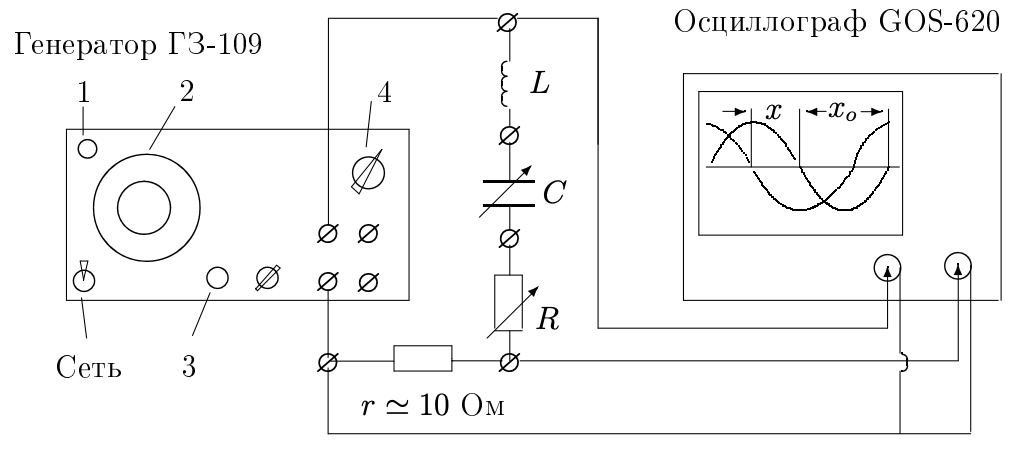
\includegraphics[scale=0.8]{image_1.png}
	\caption{Схема установки для исселдования сдвига фаз между током и напряжением}
	\label{fig:image_1}
\end{figure}

Сигнал, пропорциональный току, снимается сопротивления $ r $, пропорциональный напряжению с генератора. Оба сигнала подаются на универсальный осциллограф, имеющий два канала вертикального отклонения. На экране ЭО (\textit{рис. \ref{fig:image_1}}) видны две синусоиды, смещённые друг относительно друга на расстояние $ x $, зависящее от сдвига фаз между током и напряжением в цепи. \\

\indent Измерение сдвига фаз удобно проводить следующим образом:\\
\indent1) подобрать частоту развёртки, при которой на экране осциллогрфа укладывается чуть больше половины периода синусоиды;\\
\indent2) отцентрировать горизонтальную ось;\\
\indent3) измерить расстояние $x_0$ (см. \textit{рис. \ref{fig:image_1}}) между нулевыми значениями одного из сигналов, что соответствует разности фаз $\pi$;\\
\indent4) измерить расстояние $ x $ между нулевыми значениями двух синусоид и
пересчитать в сдвиг по фазе: $\psi = \pi \cdot x / x_0$. На \textit{рис. \ref{fig:image_1}} синусоиды на экране ЭО
сдвинуты по фазе на $\pi/2$\\

\newpage
На практике часто используются устройства, называемые \textit{фазовращателями}, которые позволяют изменять фазу напряжения в широких пределах $(0 < \psi < \pi)$. \\

\begin{figure}[!h]
	\begin{minipage}[h]{0.35\linewidth}
	Схема фазовращателя, применяемого в нашей работе, изображена
	на \textit{рис. 2}. Она содержит
	два одинаковых резистора $ R1 $, смонтированных
	на отдельной плате, магазин сопротивлений $ R $ и
	магазин емкостей $ C	 $
	\end{minipage}
	\hfill
	\begin{minipage}[h]{0.55\linewidth}
		\center{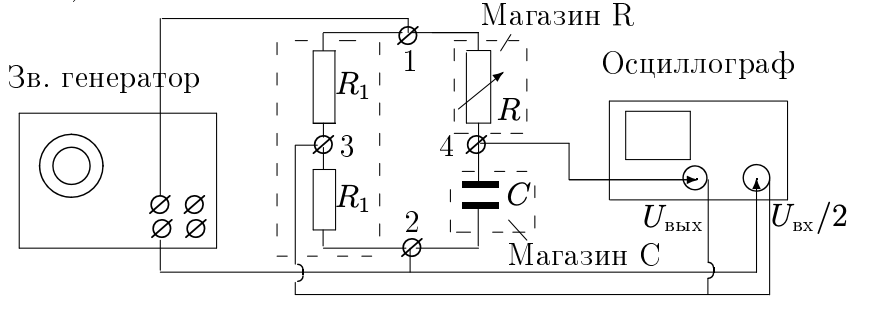
\includegraphics[width=\textwidth]{image_2} Рис. 2 Cхема установки для исследования фазовращателя}
	\end{minipage}
\end{figure}

Найдём, как зависит сдвиг фаз между входным напряжением $U_{вх} = U_0 \cos \omega t$ (точки 1 и 2 на \textit{рис. 2}) и выходным напряжением $U_{вых}$ (точки 3 и 4) от соотношения между импедансами сопротивления $R$ и ёмкости $C$. \\
Комплексные амплитуды входного и выходного напряжений связаны соотношением: \\
\[
U_{вых} = \frac{U_{вх}}{2}\frac{R + \frac{i}{\omega C}}{R - \frac{i}{\omega C}}
\]
Числитель и знаменатель полученного соотношения - комплексно-сопряжённые величины, модули которых одинаковы, поэтому амплитуда выходного напряжения не зависит от $ R $ и всегда равна $ U_0/2 $. Сдвиг фаз между входным и выходным напряжениями равен \\ 
\[
\psi = arg\frac{U_{вых}}{U_{вх}} = 2 arctg \frac{1}{\omega R C}
\]
Он может меняться от $\psi = \pi$ при $ R \rightarrow 0 $ до $ \psi = 0 $ при $ R \rightarrow \infty $

\section*{Обработка экспериментальных данных}
\begin{enumerate}
	\item Для RC-цепи построю график $ctg \psi = f(\omega C R_{\sum})$, где $R_{\sum} = R + r$ - суммарное активное сопротивление цепи
	
	\begin{figure}[h!]
		\centering
		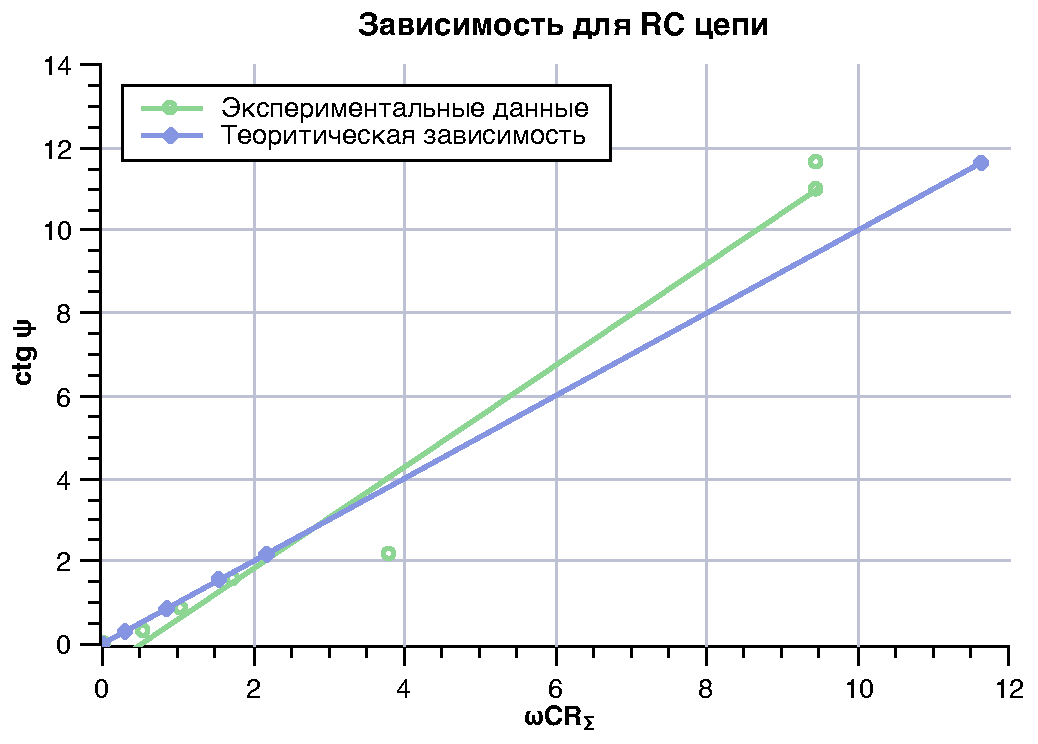
\includegraphics[width = 0.5\textwidth]{plot_1}
		\caption{График $ctg \psi = f(\omega C R_{\sum})$}
		\label{fig:plot_1}
	\end{figure}

	\newpage

	\item Для RL-цепи построю график $ctg \psi = f(R_{\sum} / \omega L)$, где $R_{\sum} = R + r + R_L$
	
	\begin{figure}[h!]
		\centering
		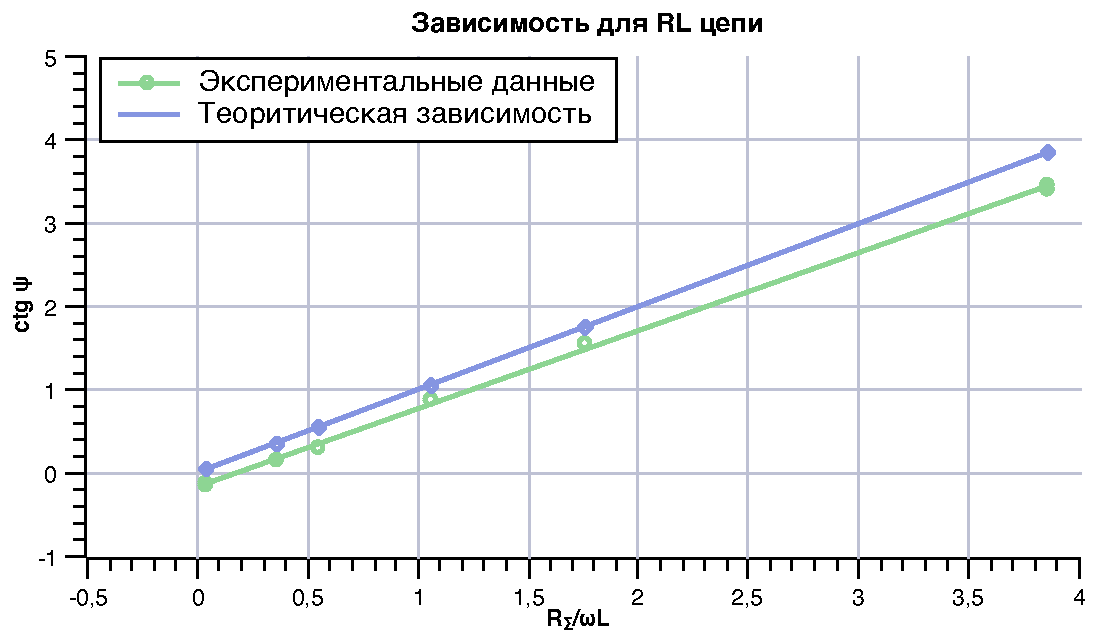
\includegraphics[width = 0.6\textwidth]{plot_2}
		\caption{График $ctg \psi = f(R_{\sum} / \omega L)$}
		\label{fig:plot_2}
	\end{figure}
	
	\item Для R = 0 и 100 Ом построю фазово-частотные характеристики контура:
	
	\begin{figure}[h!]
		\centering
		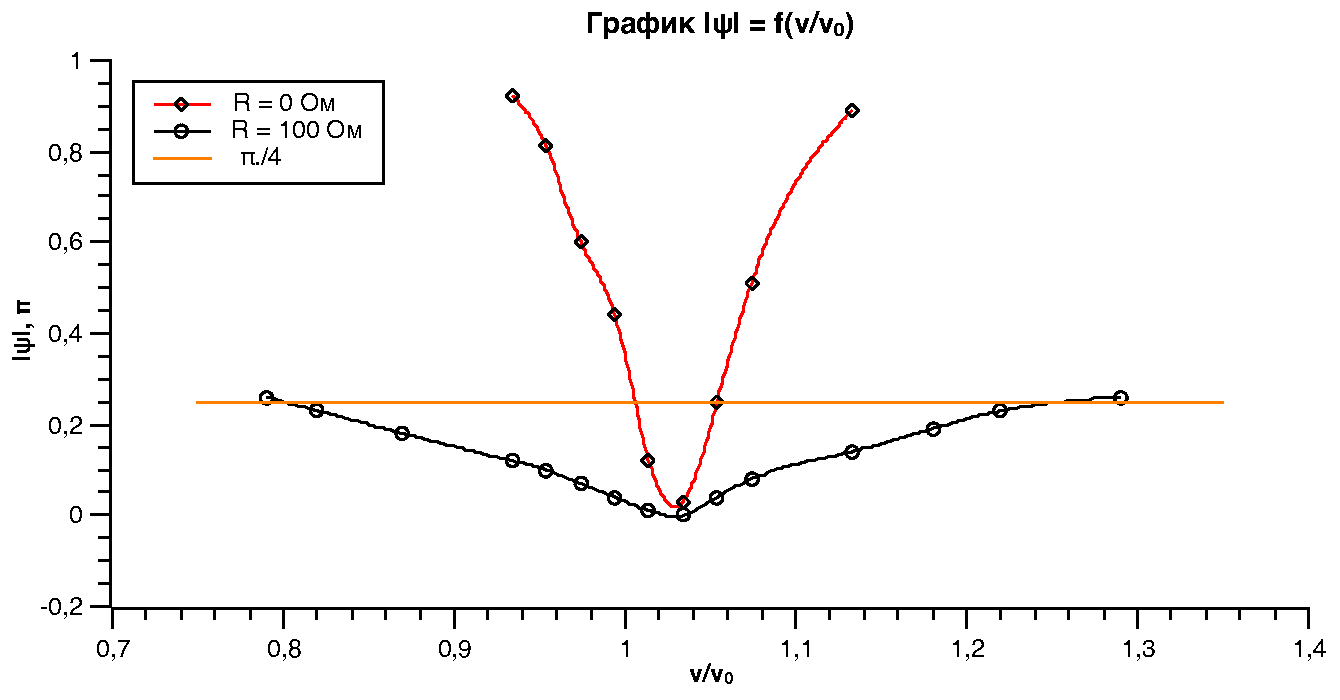
\includegraphics[width = 0.6\textwidth]{plot_3}
		\caption{График $|\psi| = f(\nu / \nu_0)$ для R = 0 Ом и R = 100 Ом}
		\label{fig:plot_3}
	\end{figure}

По данным графика: \\
\[
Q_{0 \ эксп} = 22,3 \quad \quad Q_{100\ эксп} = 2,4
\]

\item Расчитаем добротность по теоретическим данным:
\[
Q_{0 \ теор} = \frac{1}{R}\sqrt{\frac{L}{C}} \approx 25,5 \quad \quad Q_{100\ теор} = 2,8
\]
По значениям видно, что теоритические данные отличаются от экспериментальных в пределах 16 \%

\newpage
\item Построю векторную диаграмму для фазовращателя. С помощью этой диаграммы проверю экспериментально полученное  значение  сопротивления $R_M$,  при котором сдвиг фаз равен $\pi/2$

\begin{figure}[h!]
	\centering
	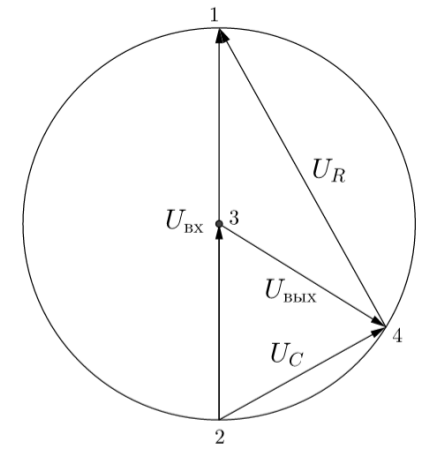
\includegraphics[width = 0.5\textwidth]{image_3}
	\caption{Векторная диаграмма фозовращателя}
	\label{fig:image_3}
\end{figure}
Разность фаз равна $\pi/2$, когда медиана 3-4 является и высотой, т.е. когда $\Delta_{124}$ - равнобедренный треугольник. \\
\[
U_C = U_R \quad \Rightarrow \quad |Z_C| = |Z_R| \quad \Rightarrow \quad R_{М \ теор} = \frac{1}{2 \pi \nu C} \approx 318 \ Ом
\]
Измеренное значение c точностью до десятых совпадает с экспериментальным:
$$
R_{M \ эксп} = 318 \ Ом
$$

\item Сведём результаты в таблицу:

\begin{table}[!h]
	\centering
	\begin{tabular}{|c|c|c|cc|cc|}
		\hline
		\multirow{2}{*}{$L_{кат}$, мГн} & \multirow{2}{*}{$R_M$, Ом} & \multirow{2}{*}{$R_{\sum}$, Ом} & \multicolumn{2}{c|}{Q}                    & \multicolumn{2}{c|}{\multirow{2}{*}{\begin{tabular}[c]{@{}c@{}}Фазовращ\\ $R_M(\psi = \pi/2)$, Ом\end{tabular}}} \\ \cline{4-5}
		&                           &                             & \multicolumn{1}{c|}{Рез. кривая} &$ f(LCR)$ & \multicolumn{2}{c|}{}                                                                                         \\ \hline
		\multirow{2}{*}{50}          & 0                         & 12,4                        & \multicolumn{1}{c|}{22,3}        & 25,5   & \multicolumn{1}{c|}{Эксп.}                                   &                   318                             \\ \cline{2-7} 
		& 100                       & 112,4                       & \multicolumn{1}{c|}{2,4}         & 2,8    & \multicolumn{1}{c|}{Теор.}                                         &       318                                   \\ \hline
	\end{tabular}
\end{table}


	
\end{enumerate}
\end{document}